%%%%%%%%%%%%%%%%%%%%%%%%%%%%%%%%%%%%%%%%%%%%%%%%%%%%%%%%%%%%%%%%%%
\documentclass[letterpaper, 10pt, conference]{ieeeconf}
\overrideIEEEmargins			% to meet printer requirements
\IEEEoverridecommandlockouts	% to override locked commands

%%%%%%%%%%%%%%%%%%%%%%%%%%%%%%%%%%%%%%%%%%%%%%%%%%%%%%%%%%%%%%%%%%
%REQUIRED PACKAGES%
\usepackage{multirow}
\usepackage{rotating}
\usepackage{float}
\usepackage{caption}
\usepackage{lipsum}
\usepackage{subcaption}
\usepackage{amsmath}
\usepackage{amssymb}
\usepackage{textcomp}
\usepackage{graphicx}
\usepackage{euscript}
\usepackage{ctable}
\graphicspath{{./Figures/}}
\usepackage[nonumberlist,acronym]{glossaries}
\usepackage[hidelinks]{hyperref}

%%%%%%%%%%%%%%%%%%%%%%%%%%%%%%%%%%%%%%%%%%%%%%%%%%%%%%%%%%%%%%%%%%

% correct hyphenation
\hyphenation{temp-orary}

% glossaries
\newacronym{ROS}{ROS}{Robot Operating System}

%%%%%%%%%%%%%%%%%%%%%%%%%%%%%%%%%%%%%%%%%%%%%%%%%%%%%%%%%%%%%%%%%%
\begin{document}

\title{Enhancing Autonomy of Mobile Robots with Behavioral Tree using ROS2}

\author{Lukas Evers$^{*,1}$, Umut Uzunoglu$^{1}$, and Ahmed Hussein$^{1}$ \textit{Senior Member, IEEE}%
    \thanks{$^{*}$ Corresponding author }%
    \thanks{$^{1}$ IAV GmbH, Berlin, Germany \newline
		{\tt\small lukas.evers@iav.de, umut.uzunoglu@iav.de, ahmed.hussein@ieee.org}}%
}

\maketitle
\pagestyle{empty}

%%%%%%%%%%%%%%%%%%%%%%%%%%%%%%%%%%%%%%%%%%%%%%%%%%%%%%%%%%%%%%%%%%

\begin{abstract}

This paper proposes a state of the art review and a behavioral planning approach to improve the autonomy of mobile robots using the Robot Operating System (ROS2). The study aims to address the issue of human intervention that is often required during the operation of autonomous mobile robots and improve the efficiency and performance of the robots. The system includes a monitoring system, sensor data storage, and behavior tree design and implementation. The effectiveness of the approach was evaluated using the Gazebo simulator, with the behavior tree handling various scenarios such as sensor failures, collisions, unreachable goals, and low battery state. The simulation results showed a significant improvement in the robot's autonomy and resilience to failures, providing evidence for the feasibility of the proposed approach. To further validate the results, additional experiments are being performed in real-world settings.

\end{abstract}

%%%%%%%%%%%%%%%%%%%%%%%%%%%%%%%%%%%%%%%%%%%%%%%%%%%%%%%%%%%%%%%%%%

\section{Introduction}
\label{sec:Introduction}

Mobile robots are increasingly being used in a variety of fields, including warehouse logistics, last-mile delivery, and agriculture. Despite being marketed as autonomous, they often require human supervision to operate correctly and are limited in their autonomy to specific environments. The Robot Operating System (ROS) is a popular platform for building and programming robots, but the standard robot still requires human intervention to ensure proper functioning and safety in uncertain environments.

This paper focuses on how behavior planning can increase the robustness and autonomy of robots running ROS2. Behavior planning allows the robot to react to failures and problems and decide on alternative courses of action to mitigate risks and achieve its goals. The paper will explore the possibility of improving current systems by adding a dedicated behavior planning component and provide an implementation of exemplary behaviors and a system architecture for incorporating behavior planning in other robots.

The study aims to demonstrate that the implementation of behavior planning can increase the robot's robustness and decrease the need for human intervention in various scenarios. The paper will present the results obtained from selected scenarios, where failures and problems will be artificially induced to test the robot's ability to behave autonomously. The paper will summarize the results and discuss the acceptance criteria for the requirements. The conclusion will provide an outlook for future work and recommendations.

%%%%%%%%%%%%%%%%%%%%%%%%%%%%%%%%%%%%%%%%%%%%%%%%%%%%%%%%%%%%%%%%%%

\section{State of the Art}
\label{sec:StateOfTheArt}

\subsection{Autonomous Driving Navigation Architectures}

Autonomous driving software architectures follow the "\textit{Sense - Think - Act}" paradigm \cite{murphy2000}, as shown in Figure \ref{fig:autonomous_driving_architecture}. Most architectures implement a hierarchical structure in which sensory inputs are processed to create an environmental representation, leading to a path from the current position to the destination computed by global planning. This is followed by behavioral planning, which ensures that the vehicle obeys traffic rules, and local planning, which translates motion commands while taking into account system constraints. An additional system monitoring layer monitors the execution of other components and triggers actions in case of failures \cite{zimmermann2020adaptive}. Vehicles can achieve (Society of Automotive Engineers) SAE levels of autonomy up to levels four and five \cite{bacha2008odin}. Expanding the behavior planning module can lead to higher levels of autonomy \cite{reke2020}.

\begin{figure}[ht]
	\centering
	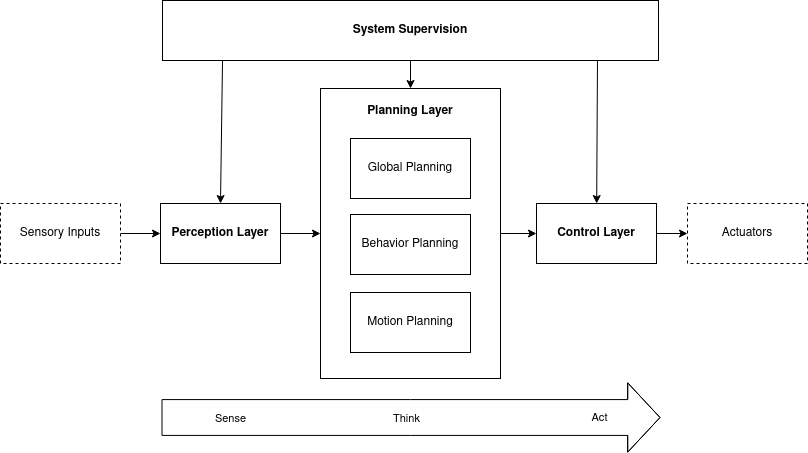
\includegraphics[width=0.9\linewidth]{Figures/autonomous_driving_architecture.png}
	\caption{Common Autonomous Driving Architecture \cite{brooks1986,velasco2020}}
	\label{fig:autonomous_driving_architecture}
\end{figure}

\subsection{Behavior Types}

The behavior planning module is responsible for choosing the best behavior to execute in a specific environment to ensure the best performance for a given task. A behavior planning approach provides the robot with acceptable behaviors for every possible scenario the robot is operating in.

\subsubsection{Reactive Approach}

The first type of behaviors implemented in behavior-based robots were reactive behaviors. This maps sensory input directly to motor commands, similar to reflexes in humans. Reactive behaviors are fast due to their low computational load, and are suitable in scenarios where real-time safety is a concern. However, a system with a solely reactive behavior planning approach will not meet requirements for higher levels of autonomy. Reactive behaviors can still be valuable in improving vehicle safety and reliability \cite{desilva2008}.

\subsubsection{Deliberative Approach}

Deliberative behaviors are defined as behaviors that involve planning and decision-making. Unlike reactive behaviors, deliberative behaviors follow the "Sense, Think, Act" paradigm and can decide the best course of action before acting \cite{murphy2000}. A behavior planner with a deliberative approach can make decisions based on current and previously processed data, and can predict environmental changes. Deliberative behaviors improve autonomy and mimic human skills, reducing the need for a human operator.

\subsubsection{Hybrid Approach}

A hybrid model combining reactive and deliberative behaviors can create reliable and intelligent systems. The hybrid approach combines the quick reaction times of reactive behaviors with the decision-making ability of deliberative behaviors, leading to more robust robots and higher levels of autonomy. The higher-level deliberative planners can override reactive planners, allowing the system to be more flexible in uncertain environments while still maintaining fast reaction times \cite{arkin1998}.

\subsection{Behavior Planning Approaches}

Robots that use a hierarchical behavior planning approach need a system to determine which behaviors to execute. Different approaches for behavior planning use states to determine which strategies and behaviors are utilized. This article presents and compares Finite State Machines (FSMs), Behavior Trees (BTs), and Partially Observable Markov Decision Processes (POMDPs).

\subsubsection{Finite State Machines}

FSMs are a popular choice for behavior planning in robotics. The fundamental idea behind FSMs is to describe behavior in terms of states that trigger actions. FSMs are defined by a set of states, a starting state, state transitions, final states, and an input alphabet. At any given time, a specific state machine is selected and its actions are executed. The benefits of FSMs include their speed and ease of implementation, especially when using libraries, which can make the development process much simpler and faster. However, as the complexity of the problem increases, so does the effort required to implement the FSM. Despite these limitations, FSMs are still a widely used approach in robotics due to their simplicity and effectiveness in controlling motors \cite{wagner2006}.

\subsubsection{Behavior Trees}

BTs are a popular approach for modeling AI for non-player characters in computer games. Unlike FSMs, BTs have a hierarchical structure, with nodes that represent actions or sequences of actions. The tree consists of a root node, child nodes, parent nodes, and leaf nodes (execution or action nodes). The behavior tree is executed by ticking the root node, which will then be recursively ticked down the tree until the execution of an action node is triggered. Control nodes, such as "Sequence," "Fallback," and "Condition," determine the order and conditions of execution for the action nodes. BTs provide a flexible and intuitive way to represent complex AI behaviors, and are widely used in the game development industry \cite{iovino2022}.

\subsubsection{Partially Observable Markov Decision Processes}

POMDPs are a more sophisticated approach for decision-making in uncertain environments. The basic idea behind POMDPs is to model decision-making as a process of choosing actions based on the probability distribution of the system's state. A POMDP consists of a set of states, actions, observations, rewards, and a transition model. POMDPs use belief states, which represent the probability distribution of the system's state, to make decisions. The solution to a POMDP is a policy, which is a mapping of belief states to actions. POMDPs are more complex than FSMs and BTs, but provide a more robust and flexible way to handle uncertainty in robotic decision-making \cite{feyzabadi2014riskaware}.

In conclusion, the behavior planning module of an autonomous driving system plays a crucial role in determining the best behavior to execute in a given environment. The behavior planning approach can range from reactive to deliberative to a hybrid of both. FSMs and BTs are two popular approaches for behavior planning in robotics, while POMDPs are a more sophisticated approach for decision-making in uncertain environments. FSMs are fast and easy to implement, while BTs provide a flexible and intuitive representation of complex AI behaviors. POMDPs are more complex but provide a robust and flexible way to handle uncertainty. The proposed approach for this study will use a BT approach for the behavior planning module, offering a hierarchical structure for modeling AI and a flexible representation of complex behaviors.

%%%%%%%%%%%%%%%%%%%%%%%%%%%%%%%%%%%%%%%%%%%%%%%%%%%%%%%%%%%%%%%%%%
\section{Proposed Approach}
\label{sec:ProposedApproach}



%%%%%%%%%%%%%%%%%%%%%%%%%%%%%%%%%%%%%%%%%%%%%%%%%%%%%%%%%%%%%%%%%%
\section{Experimental Work}
\label{sec:ExperimentalWork}



%%%%%%%%%%%%%%%%%%%%%%%%%%%%%%%%%%%%%%%%%%%%%%%%%%%%%%%%%%%%%%%%%%

\section{Results and Discussion}
\label{sec:ResultsAndDiscussion}



%%%%%%%%%%%%%%%%%%%%%%%%%%%%%%%%%%%%%%%%%%%%%%%%%%%%%%%%%%%%%%%%%%

\section{Conclusion and Future Recommendations}
\label{sec:Conclusion}


%%%%%%%%%%%%%%%%%%%%%%%%%%%%%%%%%%%%%%%%%%%%%%%%%%%%%%%%%%%%%%%%%%
%\vfill
%\section*{ACKNOWLEDGMENT}

%%%%%%%%%%%%%%%%%%%%%%%%%%%%%%%%%%%%%%%%%%%%%%%%%%%%%%%%%%%%%%%%%%
%\addtolength{\textheight}{-12cm}
%\vspace{10mm}
\bibliographystyle{IEEEtran}
\bibliography{paper}
\end{document}

%%%%%%%%%%%%%%%%%%%%%%%%%%%%%%%%%%%%%%%%%%%%%%%%%%%%%%%%%%%%%%%%%%
